
\begin{figure}[!hp]
	\centering
	\begin{minipage}[t]{0.45\textwidth}
		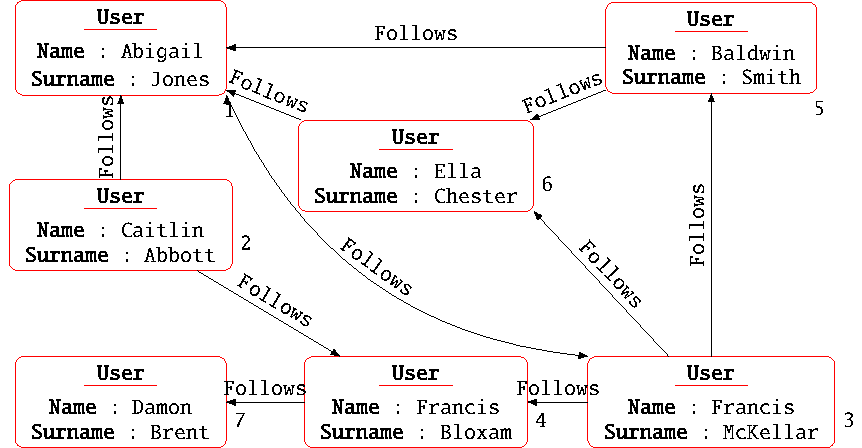
\includegraphics[width=\textwidth]{fig/04model/ex01_01}
		\subcaption{Example of a social network within the nested model: when no nesting is preformed, it appears as a usual property graph}
		\label{fig:ex0101}
	\end{minipage}\quad \begin{minipage}[t]{0.45\textwidth}
	\centering
	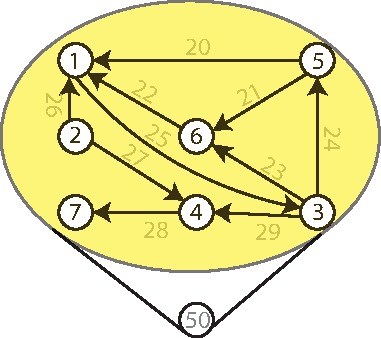
\includegraphics[width=.8\textwidth]{fig/04model/0601data}
	\subcaption{Example of nested representation of the social network data, where the whole original graph data is deliberately nested inside one vertex.}
	\label{fig:ex0103}
\end{minipage}

	\begin{minipage}[t]{0.45\textwidth}
	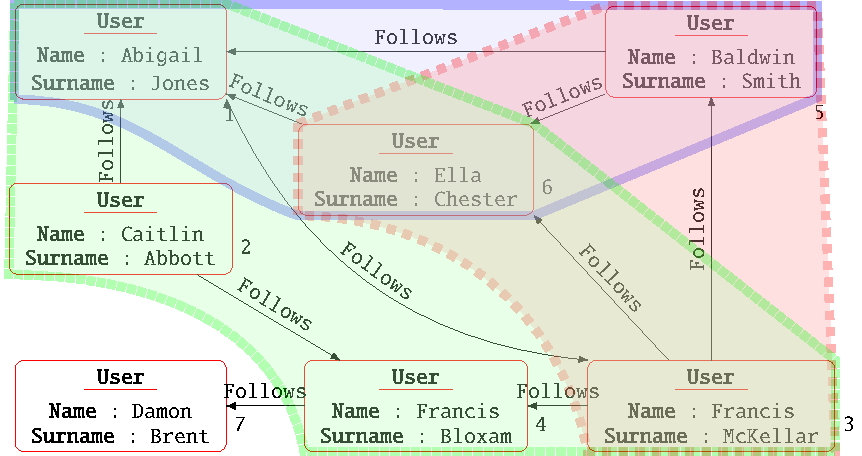
\includegraphics[width=\textwidth]{fig/04model/ex01_02}
	\subcaption{Overlapping the extracted collection of communities on top of the original social network data.}
	\label{fig:ex0102}
\end{minipage}\quad \begin{minipage}[t]{0.45\textwidth}
\centering
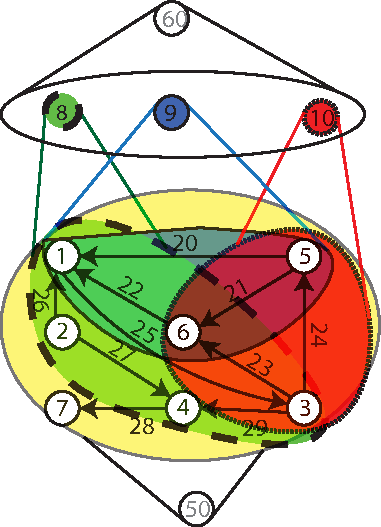
\includegraphics[width=.8\textwidth]{fig/04model/0602communities}
\subcaption{Nested representation of the communities extracted on top of the original data.}
\label{fig:ex0104}
\end{minipage}
	
	\begin{minipage}[t]{0.45\textwidth}
		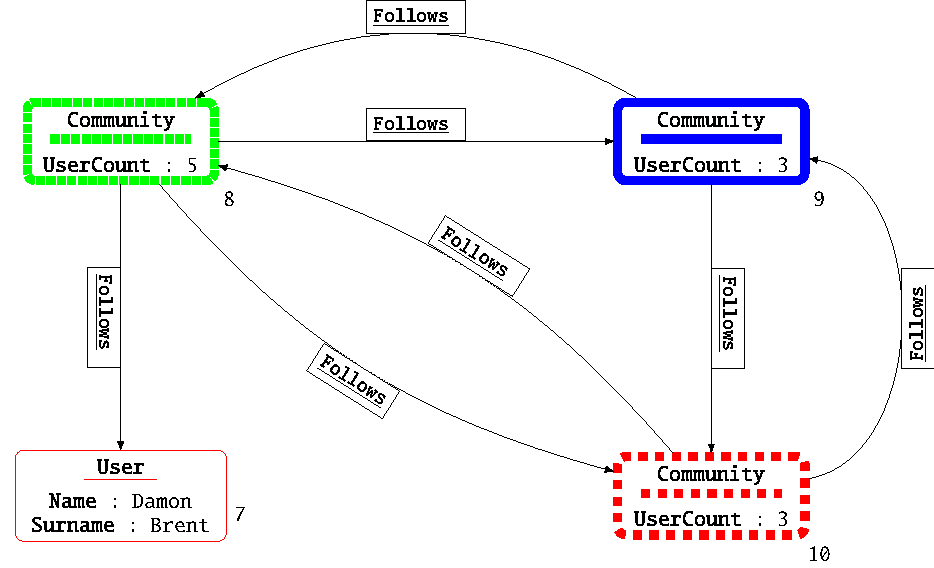
\includegraphics[width=\textwidth]{fig/04model/ex01_06}
		\subcaption{Aggregated representation of the communities, aggregated by the \texttt{COUNT} function over the vertices.}
		\label{fig:ex0106}
	\end{minipage}\quad \begin{minipage}[t]{0.45\textwidth}
		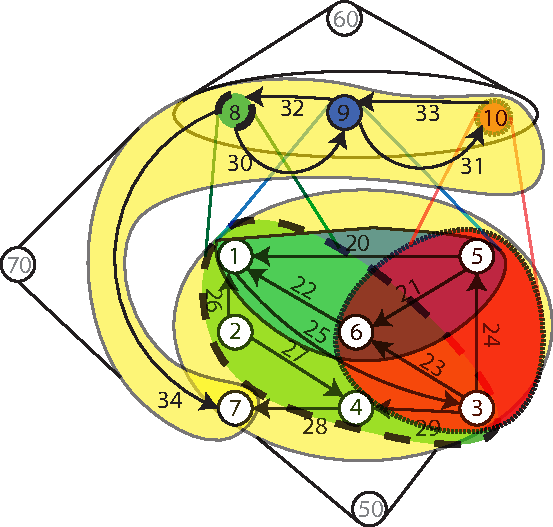
\includegraphics[width=\textwidth]{fig/04model/0603aggregation}
		\subcaption{Nested representation of the nested communities on top of the data graph.}
		\label{fig:ex0105}
	\end{minipage}
	\caption{An example of part-of aggregation within a Social Network. As we can see from the representation, property graphs cannot express the nested components. In order to ease the representation of nested graphs, edges are depicted as arcs instead of objects.}
\end{figure}


%%%%%%%%%%%%%%%%%%%%%%%%
%%%%%%%%%%%%%%%%%%%%%%%%
%%%%%%%%%%%%%%%%%%%%%%%%
%%%%%%%%%%%%%%%%%%%%%%%%
\section{Use Cases}\label{sec:squatcases}
This section will show how our proposed graph data structure can be used in different context and scenarios. We're going to show how nested graphs can be used to represent \textit{part-of} aggregations (Subsection \ref{subsec:nested-partof}) and how such data structures can be usefully used during the alignment operations (Subsection \vref{sec:ngusecases}). The usage of is-a aggregations requires to explicitly use some query languages operators, and hence this other aggregation is going to be discussed in Section \vref{subsec:representingisa}.

\subsection{Representing \textit{part-of} aggregations}\label{subsec:nested-partof}
%Given that the outline of the \textit{is-a} aggregation scenario deals with the usage of specific nested graph operators, we are going to discuss it in the next chapter at Section \vref{subsec:representingisa}. 
In the following example, we will focus on a social network use cases: we will see how a graph data representation within this model can express both aggregation that are specific to both semi-structured and relational nested models, and graphs.

\begin{example}\label{ex:partof}
	\index{part of!GSM}
	Suppose to have  asocial network graph containing millions of users, thus making impossible to visually represent the interactions happening within our data. An aggregation of this data helps us to reduce the amount of informations, and hence makes us better understand the connections within the graph. Figure \ref{fig:ex0101} represents the initial non-aggregated nested graph: given that it does not contain any nested component, it appears as an usual property graph. This graph can be expressed by our data model sketched in Figure \ref{fig:ex0103} as follows:
	
	\[SN=(50,\Set{1,\dots,7,20,\dots,29,50,101,\dots,107,111,\dots,117},\ell,\lambda,\xi,\phi)\]
	\[\phi(50,\ONTA)=[1,\dots,7]\qquad \phi(50,\RELA)=[20,\dots,29]\quad\]
	\[\forall 1\leq v\leq 7. \ell(v)=[\texttt{User}]\]
	\begin{gather*}\defSNU{1}{Abigail}{Jones}{1}\end{gather*}
	\begin{gather*}\defSNU{2}{Caitlin}{Abbott}{2}\end{gather*}
	\begin{gather*}\defSNU{3}{Francis}{McKellar}{3}\end{gather*}
	\begin{gather*}\defSNU{4}{Francis}{Bloxam}{4}\end{gather*}
	\begin{gather*}\defSNU{5}{Baldwin}{Smith}{5}\end{gather*}
	\begin{gather*}\defSNU{6}{Ella}{Chester}{6}\end{gather*}
	\begin{gather*}\defSNU{7}{Damon}{Brent}{7}\end{gather*}
	\[\forall 20\leq e\leq 29. \ell(e)=[\texttt{Follows}]\]
	\[\defSNE{e_0}{5}{1}{20}\qquad \defSNE{e_1}{5}{6}{21}\]
	\[\defSNE{e_2}{6}{1}{22}\qquad \defSNE{e_3}{3}{6}{23}\]
	\[\defSNE{e_4}{3}{5}{24}\qquad \defSNE{e_5}{1}{3}{25}\]
	\[\defSNE{e_6}{2}{1}{26}\qquad \defSNE{e_7}{2}{4}{27}\]
	\[\defSNE{e_8}{4}{7}{28}\qquad \defSNE{e_9}{3}{4}{29}\]
	Please note that vertex $50$ actually nests a full representation of a graph and consequently, we have that each vertex or edge may nest a whole graph within $\phi$.
	
%	If we want to collect all those vertices and edges and to represent them as one single vertex, then we can obtain the result in Figure \ref{fig:ex0103}. Such vertex can be then expressed within our data model as follows:
%	\[sn_0(\texttt{SocialNetwork})=(\cdot,V_{SN}\cup E_{SN})\qquad \iota(sn_0)=50\qquad \lambda(sn_0)=\Set{\texttt{Graph}}\]
%	Hereby, we can extend our previous Social Network data as follows:
%	\[\begin{split}
%	(&\Set{1,2,3,4,5,6,7,sn_0},\Set{e_0,\dots,e_9},\\
%	&\Set{\texttt{Name},\texttt{Surname},\texttt{SocialNetowrk}},\Set{\texttt{User},\texttt{Follows},\texttt{Graph}},\ell,\lambda,\iota)
%	\end{split}\]
%	Please note that the information content is preserved because id references to the original vertices are used. 
By using community detection algorithms, we extract a set of graph collections in polynomial time \cite{vanDongen2012}, where some overlaps between communities may be present. Figure  \ref{fig:ex0102} presents such extracted communities as shaded areas on top of the original data sources: please note that the property graph model does not allow to represent such communities inside the same given graph. This problem can be overcame by our proposed data structure as showed in Figure \vref{fig:ex0104}: each community, marked with a different color, is nested inside one given object. In particular we have that:
	
	\[\phi(8,\ONTA)=[1,2,3,4,6]\quad \phi(8,\RELA)=[22,23,25,26,27,29]\]
	\[\phi(9,\ONTA)=[1,5,6]\quad \phi(9,\RELA)=[20,21,22]\]
	\[\phi(10,\ONTA)=[3,5,6]\quad \phi(10,\RELA)=[21,23,24]\]
	As we can see from the same picture, we can create a graph collection by creating another object including the three objects nesting the communities:
	\[\ell(60)=\Set{\texttt{Communities'Collection}}\qquad \phi(60,\ONTA)=[8,9,10]\]
	The aggregation function evaluating how many users are contained within the community can be expressed with a \texttt{script} expression as follows:
	\[\ell(8)=\ell(9)=\ell(10)=\{\texttt{Community},\texttt{UserCount}\}\]
	\[\xi(8)=\xi(9)=\xi(10)=[\textup{\color{webgreen}``}\scriptline{0+(o.phi ["Entity"])}\textup{\color{webgreen}''}]\]
	Please observe that each expression in $\xi(o)$ is going to be evaluated by choosing ``\scriptline{o}'' as $o$.
	
	
%\textit{	Among all the communities, we can represent the one where only ``Francis Bloxam'' is represented as the following nested vertex: 
%	
%	\[c_1(\texttt{Community})=(\cdot,[1,2,3,4,6,22,23,24,26,27])\qquad \iota(c_1)=8\qquad \lambda(c_1)=\Set{\texttt{Graph}}\]
%	
%	We can do similarly for all the other communities. In order to express the graph collection within vertex $\iota(v_0)=60$, we can either store each different community within one distinct attribute ($opt_1$), or define $v_0$ as a single-attributed vertex containing the graph of all the other communities ($opt_2$). The two different solutions are then provided as follows:
%	\[opt_1(\texttt{1})=(\cdot,[1,2,3,4,6,22,23,24,26,27])\qquad opt_1(\texttt{2})=(\cdot,[3,6,5,21,23,24])\]
%	\[opt_1(\texttt{3})=(\cdot,[1,5,6,20,21,22])\qquad \lambda(opt_1)=\Set{\texttt{GraphCollection}}\]
%	
%	
%	\[opt_2(\texttt{Communities})=(\cdot,[8,9,10])\qquad \lambda(opt_2)=\Set{\texttt{GraphOfGraphs}}\]
	As a result, we would like to summarise each component as a single vertex containing all the vertices and edges describing the communities, as represented by Figure \ref{fig:ex0106}, where only the result of the aggregation is provided. Given the outline provided by the former example, it is easy to define a preliminary algorithm that takes both the outcome of the community detection algorithm and the social network graph, and aggregates each community as a single vertex: 
	\begin{alphalist} 
		\item \label{aggrphase:a} given a graph with its vertex set $V$, return as $V'$ the vertices that do not appear within any detected community, 
		\item \label{aggrphase:b} alongside with the aggregated representation of each community.
	\end{alphalist}
	As a result of this vertex creation phase, vertices $8$, $9$ and $10$ are selected alongside with $7$, which does not belong to any community. As a result we have that:
	\[\phi(70,\ONTA)=[7,8,9,10]\]
	In a later step, we must also define the criteria by which we have to generate the edges among the $V'$ returned vertices. In particular, we must consider that new edges may occur between vertices where:
	\begin{mylist}
		\item source comes from phase \ref{aggrphase:a} and targets from \ref{aggrphase:b} (or vice versa),
		\item or if vertices from phase \ref{aggrphase:a} are linked to at least one vertex appear inside an aggregated component from \ref{aggrphase:b} (or vice versa),
		\item or even if one vertex from phase \ref{aggrphase:b} contains a vertex that is linked to another vertex represented inside an aggregated component from \ref{aggrphase:b}
	\end{mylist}. If we want to simply establish a link for all the aforementioned cases, then the result can be modelled within our nested graph definition. 

The result of such aggregation is depicted by the nested element $70$, containing both the vertices and the edges extracted following the previous sketched algorithm.
\[\phi(70,\RELA)=[30,31,32,33,34]\]
%In order to express $70$ as a nested graph, we can use the previously defined transformation function.
\end{example}


Given that edges can also contain graph nested components, we could also decide that each edge obtained after the vertex aggregation phase can show how many users (vertices) are shared between the two communities and provide which vertices and edges from the source and target communities allowed the creation of the new link. As we can observe from this latter description, we have that the graph collections required to perform the nesting can be returned by an external algorithm, while the link creation process can be derived from a previous pattern matching process on top of the previously vertex aggregated data. On the other hand, since current graph traversal and graph pattern matching languages do not formally support nested graphs, it is impossible to use currently implemented languages to express the vertex containment. On the next chapter we will then discuss on the features that are required by the graph query languages on top of this novel data structure.


